\documentclass{standalone}
\usepackage[T1]{fontenc}
\usepackage[latin2]{inputenc}
\usepackage[english]{babel}
\usepackage{tikz}
\usepackage{times}
\usetikzlibrary{calc,through,backgrounds,positioning,fit}
\usetikzlibrary{shapes,arrows,shadows}
 
\begin{document}
 
 
\centering
\begin{tikzpicture}
\node (n2) [stt] at (-2,0) {
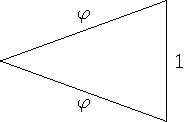
\includegraphics[scale=0.5]{zad5-10c.pdf}
};
\node (n2) [stt] at (2,0) {
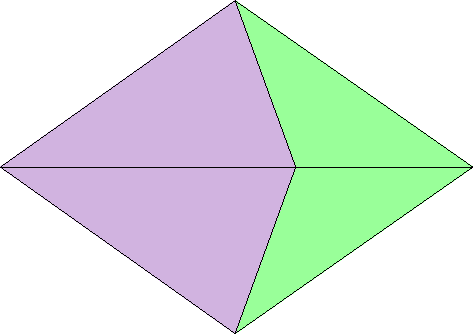
\includegraphics[scale=0.3]{zad5-10d.pdf}
};
\node (n2) [stt] at (-2,-2) {
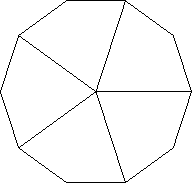
\includegraphics[scale=0.7]{zad5-10.pdf}
};

\node (n2) [stt] at (2,-2) {
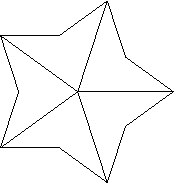
\includegraphics[scale=0.6]{zad5-10b.pdf}
};




\end{tikzpicture}

 
\end{document}